% 05-unsupervised-learning-clustering.tex

% Unsupervised Learning – Clustering
% 5.1. Introduction: Provides an overview of the clustering task and its objectives.
% 5.2. Determine the Number of Clusters: Uses methods like the elbow method or silhouette analysis to determine the number of clusters.
% 5.3. Hyperparameter Tuning: Tunes other hyperparameters, if any.
% 5.4. Cluster Visualization: Visualizes the clusters through t-SNE.
% 5.5. Cluster Analysis: Analyzes the characteristics of each cluster.
% 5.6. Intent Homogeneity: Assesses if clusters reflect intent division.
% 5.7. Specific Attack Categories: Associates clusters with specific attack categories.

% Section Title
\section{UNSUPERVISED LEARNING - CLUSTERING}

    % Main Content

    \subsection{Introduction}
    
        Unsupervised learning, a powerful branch of machine learning, was applied in this project to gain insights from SSH attack data. The primary focus was on leveraging clustering methods to group similar attack sessions based on their intrinsic patterns and characteristics. By analyzing these groups, the study aimed to uncover hidden relationships and categorize different attack intents and behaviors without relying on predefined labels. 
    
    \subsection{Data Preparation}
    
        The dataset chosen was the one generated through the TF-IDF vectorization technique. This was made because it was essential to start with a dataset that represented in the best way the frequency and the importance of words, making each word as a dimension of our vector.

    \subsection{Clustering Methods}
    
        Clustering techniques were employed to uncover natural groupings within the dataset, providing insights into SSH attack patterns. The following methods were used:
        
        \begin{itemize}
        
            \item \textbf{K-Means Clustering}: The Elbow Method was applied to determine the optimal number of clusters by examining the total within-cluster sum of squares (inertia). Silhouette scores were also calculated to evaluate the cohesion and separation of clusters.
            
            \item \textbf{Gaussian Mixture Model (GMM)}: Unlike K-Means, GMM considers the probability of each data point belonging to a cluster, providing a more flexible and nuanced clustering approach. The optimal number of clusters was determined using a combination of log-likelihood scores, which measure how well the model fits the data, and silhouette analysis to validate cluster quality.
            
        \end{itemize}
        
    \subsection{Clustering Evaluation Techniques}
    
        \subsubsection{K-Means Clustering \\}
            
            The Elbow Method graph (Figure~\ref{fig:kmeans_elbowmethod}) shows a steep decline in clustering error between 3 and 6 clusters, followed by a more gradual decrease as the number of clusters increases. The point of inflection, or "elbow," appears around 6 clusters, suggesting that adding more clusters beyond this point results in diminishing improvements in minimizing intra-cluster variance. The Silhouette Score graph exhibits a rapid increase up to 5 clusters, reaching a stable high value of approximately 0.95. A drop is observed around 8 clusters, after which the score gradually increases again, peaking beyond 12 clusters. Considering both metrics, the optimal number of clusters for K-Means is likely between 5 and 6, ensuring a trade-off between clustering accuracy and computational efficiency.
        
        \subsubsection{Gaussian Mixture Model (GMM) \\}

            The Silhouette Score graph shows a sharp increase up to 5 clusters, reaching a stable high value around 0.95. A slight drop is observed at 8 clusters, followed by a steady increase, with the highest scores occurring beyond 12 clusters. This suggests that increasing the number of clusters generally improves separation and cohesion, though the optimal balance appears to be around 6 clusters, where the highest stable performance is first achieved. The Log-Likelihood Score graph indicates a rapid increase from 3 to 5 clusters, after which the improvements become more gradual. Beyond 12 clusters, the score stabilizes, indicating diminishing returns in model fitting. Considering both metrics, an optimal cluster configuration is likely between 6 and 8 clusters, balancing cluster separation, model likelihood, and computational efficiency.

        % \vspace{-0.3cm}
        
        \begin{figure}[h]
            \centering
            \begin{minipage}[c]{0.47\textwidth}
                \centering
                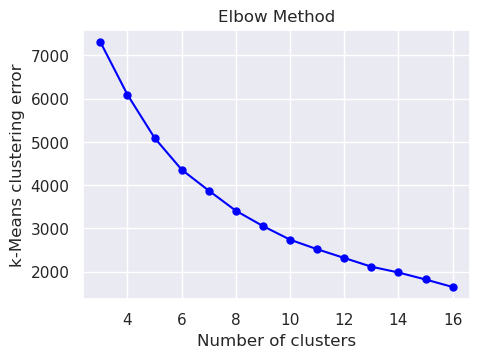
\includegraphics[width=\textwidth]{../figures/plots/section3/k-means_clustering_error.png}
                \caption{K-means Elbow Method}
                \label{fig:kmeans_elbowmethod}
            \end{minipage}
            \hfill
            \begin{minipage}[c]{0.47\textwidth}
                \centering
                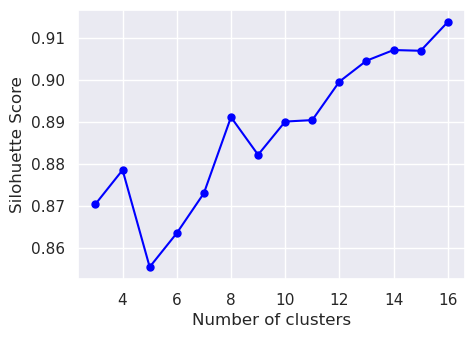
\includegraphics[width=\textwidth]{../figures/plots/section3/k-means_silohuette_score.png}
                \caption{K-means Silhouette Score}
                \label{fig:kmeans_silhouette_score}
            \end{minipage}
        \end{figure}
        
        % \vspace{-0.5cm}
        
        \begin{figure}[h]
            \centering
            \begin{minipage}[c]{0.47\textwidth}
                \centering
                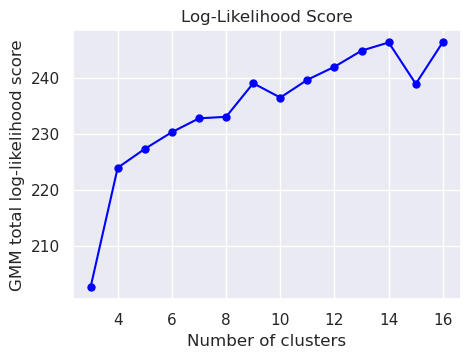
\includegraphics[width=\textwidth]{../figures/plots/section3/gmm_total_log-likelihood_score.png}
                \caption{GMM Log-Likelihood Score}
                \label{fig:gmm_log_likelihood}
            \end{minipage}
            \hfill
            \begin{minipage}[c]{0.47\textwidth}
                \centering
                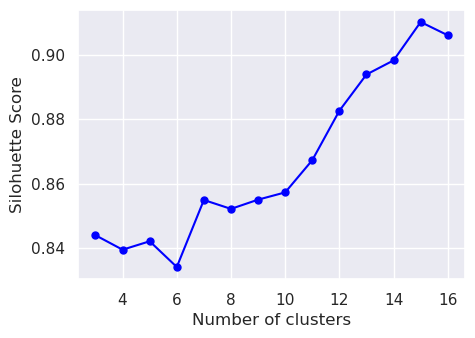
\includegraphics[width=\textwidth]{../figures/plots/section3/gmm_silohuette_score.png}
                \caption{GMM Silhouette Score}
                \label{fig:gmm_silhouette_score}
            \end{minipage}
        \end{figure}

    \subsection{Hyperparameter Tuning}
    
    To optimize both the K-Means and Gaussian Mixture Model (GMM) clustering approaches, hyperparameter tuning was performed using grid search with cross-validation. For K-Means clustering, the optimal parameters identified were:
    \begin{table}[h]
        \centering
        \begin{tabular}{|c|c|c|}
            \hline
            \textbf{Initialization method} & \textbf{Number of initializations (n\_init)} & \textbf{Maximum iterations (max\_iter)} \\
            \hline
            k-means++ & 10 & 50 \\
            \hline
        \end{tabular}
    \end{table}

    The final clustering results achieved a silhouette score of 0.9490 and an inertia value of 1708.96. The high silhouette score indicates well-defined and well-separated clusters, while the minimized inertia suggests an efficient clustering structure. For the Gaussian Mixture Model (GMM), the best hyperparameters found were:
        
        \begin{table}[h]
            \centering
            \begin{tabular}{|c|c|c|c|}
                \hline
                \textbf{Covariance Type} & \textbf{Initialization method} & \textbf{Maximum iterations (max\_iter)} & \textbf{Tolerance (tol)} \\
                \hline
                full & k-means & 50 & 0.001 \\
                \hline
            \end{tabular}
        \end{table}

    The model's performance was evaluated using a silhouette score of 0.9398 and a log-likelihood score of 508.71. Both clustering techniques provided effective segmentation of the dataset. K-Means exhibited a slightly higher silhouette score, suggesting better-defined cluster boundaries, while GMM’s higher log-likelihood highlights its ability to model complex, overlapping clusters.
    \subsection{Clusters Visualization}
    
        To better understand the structure of the clusters, t-SNE dimensionality reduction was applied. While t-SNE is effective for visualizing high-dimensional data, its interpretation must align with clustering validation metrics. 
        
        \begin{figure}[h]
            \centering
            \begin{minipage}[c]{0.47\textwidth}
                \centering
                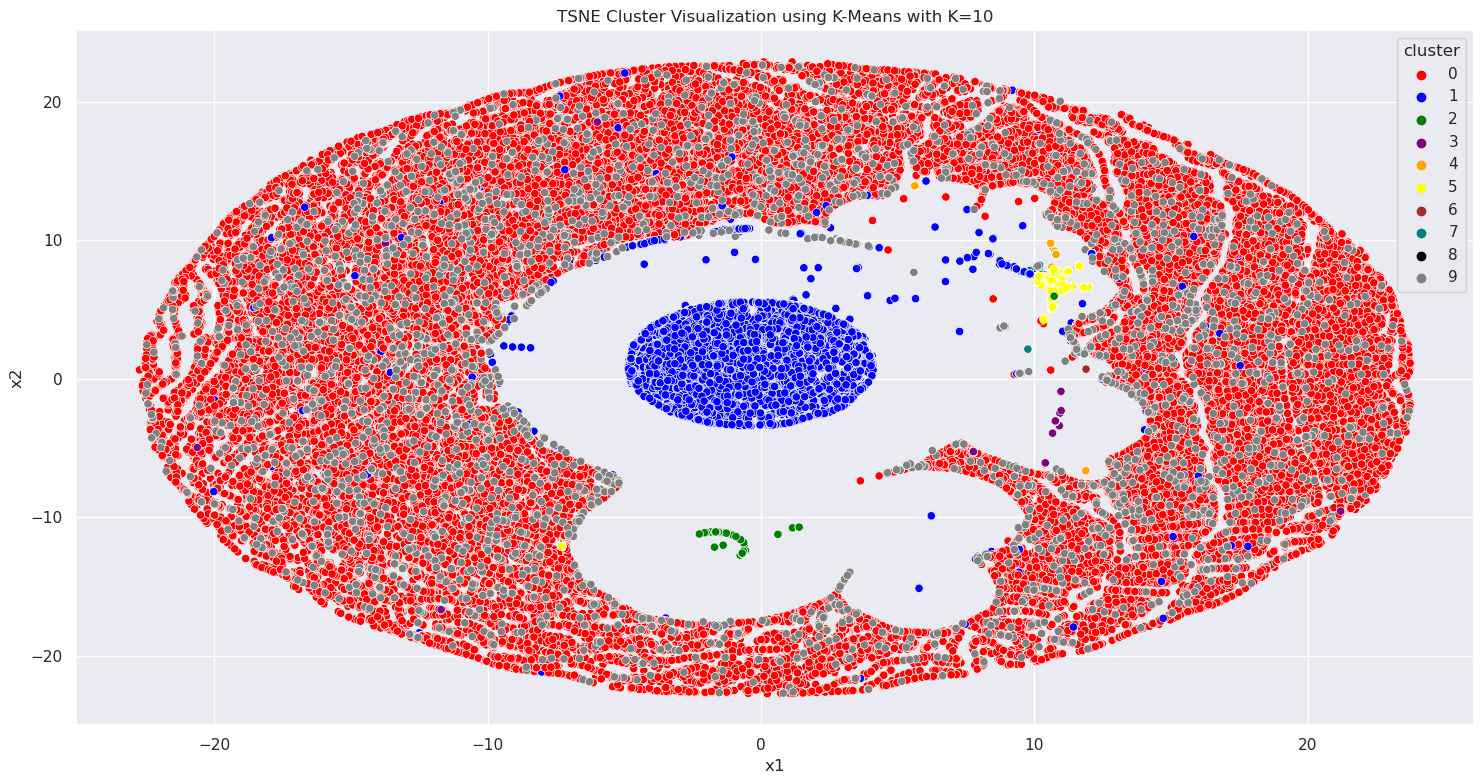
\includegraphics[width=\textwidth]{../figures/plots/section3/tsne_kmeans_clusters.png}
                \caption{t-SNE Visualization of K-Means Clusters}
                \label{fig:tsne_kmeans}
            \end{minipage}
            \hfill
            \begin{minipage}[c]{0.47\textwidth}
                \centering
                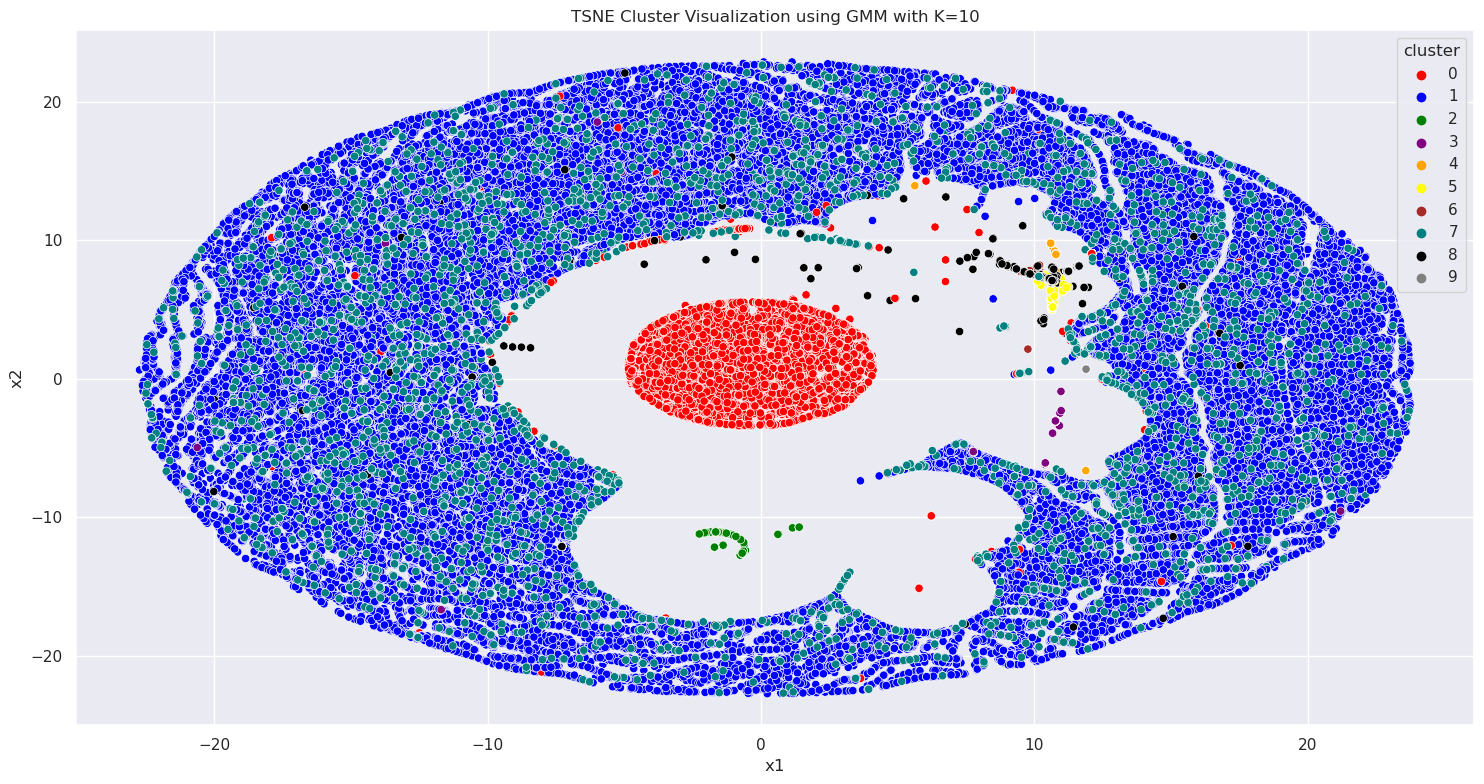
\includegraphics[width=\textwidth]{../figures/plots/section3/tsne_gmm_clusters.png}
                \caption{t-SNE Visualization of GMM Clusters}
                \label{fig:tsne_gmm}
            \end{minipage}
        \end{figure}

        \subsubsection{K-Means Visualization \\}

        The t-SNE visualization of K-Means clustering reveals that a significant portion of the dataset is assigned to a dominant red cluster. While this cluster appears dense, it raises concerns about the method’s ability to differentiate between distinct attack types. The blue and purple clusters are more compact and well-separated, suggesting a few meaningful subgroups. However, several smaller clusters are sparsely distributed, potentially indicating outliers rather than well-formed attack patterns. This visualization suggests that a majority of attacks are grouped together, limiting the effectiveness of this approach.

        \subsubsection{GMM Visualization \\}
        
        The t-SNE visualization of GMM clustering reveals a different structure. Unlike K-Means, which forces strict cluster assignments, GMM probabilistically associates data points with multiple clusters. The resulting visualization displays smoother transitions between clusters, particularly in peripheral areas. However, a large central cluster remains dominant, similar to K-Means. This suggests that while GMM captures more complex attack distributions, it does not necessarily provide significantly better differentiation between attacks. The presence of overlapping points implies that GMM is better suited for identifying gradual variations in attack behaviors rather than strict categorization.

    \subsection{Clusters Analysis}

        \subsubsection{Word Cloud Representation \\}

        Word clouds were generated to highlight the dominant terms in each cluster. However, upon closer inspection, the clusters display a significant degree of overlap in command usage, which raises concerns about the distinctiveness of the attack groupings.
        \begin{itemize}

            \item Many clusters contain commonly used system commands such as \texttt{grep}, \texttt{tmp}, and \texttt{var}, which are present in multiple clusters. This suggests that the clustering process may have grouped sessions based on general command usage rather than clear behavioral differences in attack methodologies. While some clusters, such as Cluster 4 with \texttt{ssh}, \texttt{authorizedkeys}, and \texttt{passwd}, appear indicative of authentication-related activity, most clusters contain highly generic commands that do not necessarily indicate distinct attack types.
            
            \item Clusters 5 and 8, which feature \texttt{chmod}, \texttt{wget}, and \texttt{rm}, could suggest interactions with file systems and downloading behaviors. However, these commands are widely used across many attack types, reducing their effectiveness in defining specific attack categories.
            
            \item Cluster 2, which includes \texttt{busybox} and \texttt{mounts}, is one of the few clusters that might point toward IoT-related attack scenarios, as these commands are frequently used in embedded system environments. However, without additional contextual information, this distinction remains speculative.
            
            \item Cluster 6 contains \texttt{shell}, \texttt{system}, and \texttt{name}, but these terms are too generic to draw meaningful conclusions about a particular type of attack.
            
        \end{itemize}
        Overall, while word clouds provide a useful summary of frequent commands, they do not strongly support the hypothesis that the clusters correspond to clearly defined attack patterns.
            
            \begin{figure}[H]
                \centering
                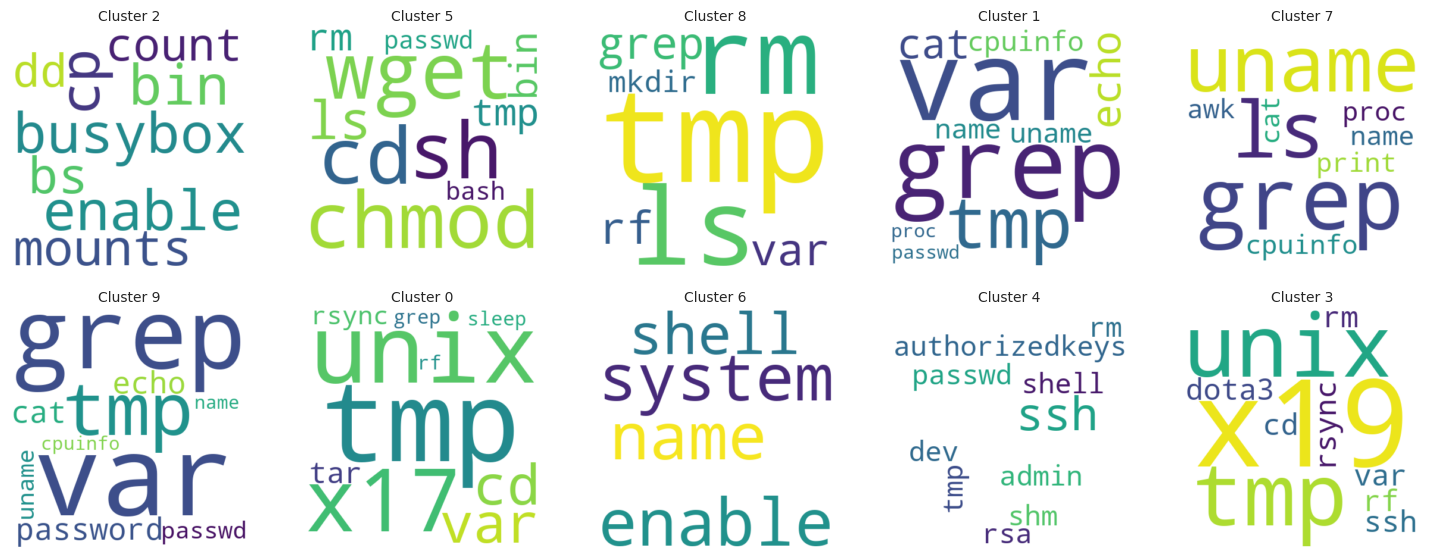
\includegraphics[width=0.9\textwidth]{../figures/plots/section3/circular_wordclouds.png}
                \caption{Word Clouds for Each Cluster}
                \label{fig:word_clouds}
            \end{figure}
            
            \subsubsection{Community Detection \\}
            
                Graph-based community detection was applied to further segment clusters into subgroups. The results indicate that specific communities focus on distinct attack behaviors:

                \begin{itemize}
                    \item The K-Means-based community detection identified well-defined subgroups, but many commands appear across multiple communities, indicating overlapping behaviors.
                    \item The GMM-based community detection aligns with K-Means results, with some additional flexibility in capturing transitional attack patterns. However, the persistence of a dominant cluster in both methods suggests that neither approach fully separates attacks into meaningful, non-overlapping categories.
                \end{itemize}
                
                Overall, while community detection adds another layer of granularity, the results indicate that SSH attack behaviors exhibit significant overlap, making strict segmentation challenging. Additional analysis of the single communities in the appendix. 
                Instead, the overlap in dominant terms suggests that the clustering process may have captured broader system interaction behaviors rather than distinct categories of SSH attack tactics.
                \begin{figure}[h]
                    \centering
                    \begin{minipage}[c]{0.47\textwidth}
                        \centering
                        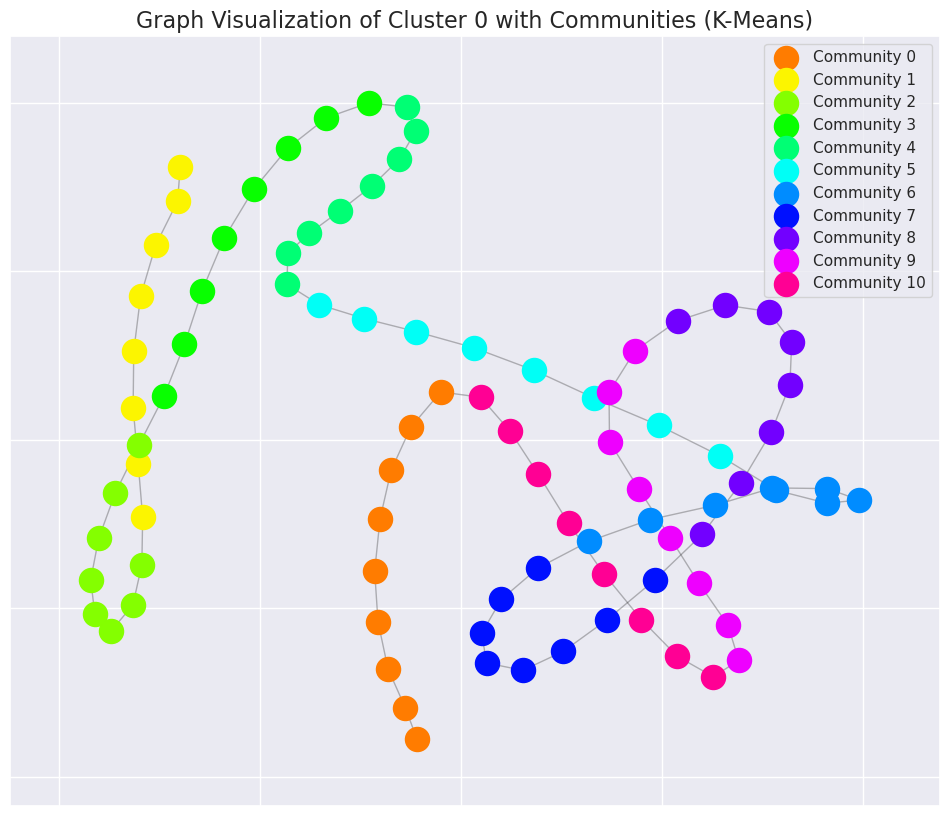
\includegraphics[width=0.8\textwidth]{../figures/plots/section3/k-means_graph_visualization_of_cluster_0_with_communities.png}
                        \caption{Community Detection in Cluster 0 (K-Means).}
                        \label{fig:kmeans_graph}
                    \end{minipage}
                    \hfill
                    \begin{minipage}[c]{0.47\textwidth}
                        \centering
                        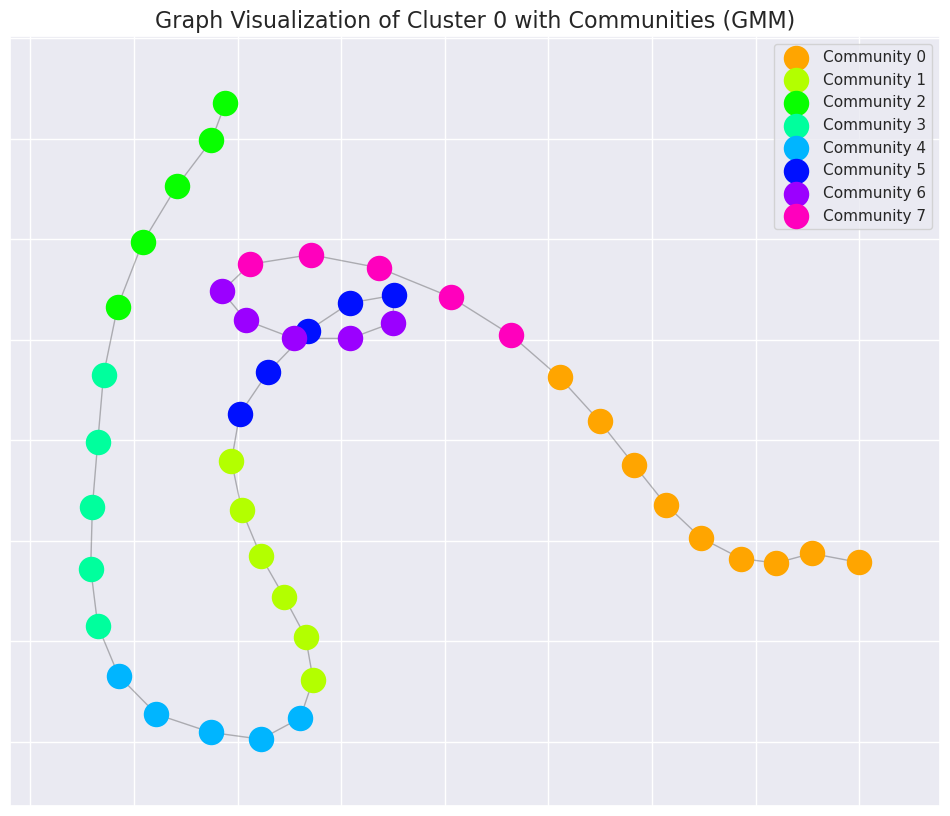
\includegraphics[width=0.8\textwidth]{../figures/plots/section3/gmm_graph_visualization_of_cluster_0_with_communities.png}
                        \caption{Community Detection in Cluster 0 (GMM).}
                        \label{fig:gmm_graph}
                    \end{minipage}
                \end{figure}
            

    \subsection{Conclusion}
        

        This analysis provided insights into SSH attack patterns through clustering, using both K-Means and GMM. While validation metrics and hyperparameter tuning optimized the models, the visualized results indicate significant overlap between clusters, suggesting challenges in achieving well-separated attack groupings. The presence of dominant clusters encompassing much of the dataset hints at either insufficient feature discrimination or limitations in the chosen clustering techniques. Despite these challenges, the study demonstrates the potential of unsupervised learning in revealing underlying structures in SSH attack data, forming a basis for further refinement in cybersecurity threat detection.
        